%!TEX root = ../../super_main.tex

\section{Background Sensor Service}
\label{sec:background_sensor_service}

\todo[inline]{Skriv en fluff introduktion der beskriver motivationen for at samle dataen på en baggrundstråd. Please lad være med at nævne noget i mono tak}

\subsection{Android Services}
\todo[inline]{Skriv hvorfor vi har valgt at bruge en service -> memory/power optimering. Det skal være NEMT at forstå. Knapt så meget generelt snak, og mere konkret hvad vi har behov for, og hvorfor.}

A service in Android is an application component which encapsulates long running background task. A service can run in the same process as the graphical interface shown to users, but also in a separate process. Running the service separately is ideal for data collection, since we do not have to allocate memory for GUI elements when they are unnecessary. Services have their own lifecycles and can be configured in many different ways. They can be configured as an API where the service itself has a short lifespan while serving some data or while performing a short task or they can be configured as a long running background task with its own complex behavior.
\\\\
% Message parsing
The Android framework supports two-way message parsing as a way of communication with a service when it runs in a different process. Message parsing makes it easy for the Android \mono{Activity} elements in the graphical and interactive part of the application to communicate with our \mono{BackgroundSensorService}.

% Boot receiver
% On Application start
\subsection{Service Start}
\label{sub:service_start}
Our \mono{BackgroundSensorService} should ideally always be running, which does not imply that it is constantly using processing resources. We have implemented two measures to ensure that the service is running for as much time as possible. The first measure is an Android \mono{BroadcastReceiver}, which upon receiving a system wide \emph{boot completed}-broadcast, starts the service. The second measure involves attempting to start the service every time the graphical application is started. It will, however, not start if it is already running.

\subsection{Snapshot Generation and Upload}
\label{sub:background_sensor_service_snapshot_generation_and_upload}

\todo[inline]{Lav en ordentlig intro. Inspiration: Referer tilbage sig noget med: ``For at vi kan lave snapshots som covered i section bla skal vi sætte en timer der kan håndtere sensor providers igang der kan sige nu skal vi måle.''}

The background service uses an independent timer for snapshot generation. The timer for snapshot generation is encapsulated in a class called \mono{SnapshotTimer}, which is started whenever the service has an active running campaign. Tasks, which utilizes our sensor providers to generate snapshots, are then scheduled by this timer at a constant rate, until the campaign is completed or stopped by the participant.
\\\\
Before we send all generated snapshots to the server we transform them to a JSON format. We have chosen to utilize the JSON format because it is human readable, making it easier for us to debug; it is decent for machine learning purposes; and it is a common format which natively can be interpreted by the PHP code on our server. Choosing JSON is in this way convenient, however it is at the sacrifice of spending extra bandwidth for sending the data, which is rather inconvenient for the participants. A better solution would be to use some format with few-to-no keys, where we have optimized how much space we use. 
\\\\
When we have converted the data to JSON, the actual upload of snapshots is done separately and is encapsulated in a class called \mono{SynchronizationManager}. The upload should ideally be done using as little network resources as possible, and thereby also reduce power and bandwidth consumption. 
\\\\
\todo[inline]{Her er en teknisk detalje (spørg Marhlder), som skal skrives ind i overstående. Det skal nok ikke forklares så meget i dybden. Fortæl istedet hvad en threadpool er, og hvad vi får ud af at bruge den! 
% indsæt newline her
The \mono{BackgroundSensorService} is configured to have one thread available per sensor type, i.e. per \mono{SensorProvider} specialization (see \secref{sub:providing_sensor_data_implementation}), used in the service. This lets the scheduling of the gathering from the different \mono{SensorProvider} instances up to the underlying Java implementation of threads in a hope to run the different types of sensors and other data sources as independently as possible. Data is only collected from the \mono{SensorProvider} instances if the corresponding sensors are included in the currently active campaign and if the system is currently gathering a snapshot. There is no data collection activity in the \mono{BackgroundSensorService} unless a timed task for a snapshot is running. 
% indsæt newline her
CPU resources, and thereby battery, are therefore only consumed on demand. We do not provide any real time guarantees but the different threads from the different streams of data should always be able to run unless they get starved by other processes in the system. Temporary starvation of the data collecting threads might result in missed updates from different data sources.}

\todo[inline]{Omskriv følgende paragraf til at beskrive hvad vi har gjort, og hvad vi har brugt den til konkret. Start med at forklare problemer med kommunikation over netværk (ref til general strategies i problem analysen). jvf. Holms rettelser, så brug gerne: The \mono{GCMNetworkManager} incorporates radio based optimizations and will start all the pending tasks if the radio is active and a minimum time, specified by the parameters, has elapsed. This minimizes unnecessary wake-ups of the radio and thus minimizes battery consumption}

An example of an Android API, or rather a library with Google APIs for Android, which could help optimize network usage, and the, would be the \mono{GCMNetworkManager}, which is an Android service, that can schedule encapsulated network tasks. \mono{GCMNetworkManager} \parencite{gcmnetworkmanager} handles batching of network tasks; retries; backoffs, in case a remote server is not responding or is busy; waiting for Wi-Fi, for bandwidth heavy communication; waiting with communication until the device is charging; and waiting until a radio becomes active, for instance by getting activated by another application. It does all of this based on parameters given to every encapsulated network tasks such as a desired time frame for the network communication and desired network or battery conditions.  
\\\\
Our \mono{SynchronizationManager} uses the \mono{GCMNetworkManager} to schedule a periodic task which attempts to upload gathered snapshots to the server. Our periodic task is configured to override the old pending tasks if it is rescheduled, but has not yet been executed. It is then up to the \mono{GCMNetworkManager} to determine when the task should be executed based on parameters specified when the task is defined. Our task is configured to require that an unmetered connection, e.g. Wi-Fi, is available before the task can be executed, since participants might not be willing to pay for data transfer of the snapshots. 
\\\\
Using \mono{GCMNetworkManager} makes sense for network related operations, which can be delayed in order to minimize battery consumption. Other network tasks which should happen instantly, such a refreshing the GUI with lists of campaigns from the server, are therefore not applicable to be optimized with \mono{GCMNetworkManager}. 

\subsection{Concurrency Overview}
We have attempted to give an overview of the current processes and threads running in the mobile application in \figref{fig:system_currency_and_lifecycle} illustrated with an activity diagram. We provide this overview so the communication between the different processes and communication in the application becomes more clear.
\\\\
As seen in the figure the system is split into two parts, namely an \emph{Android Application Process} part (GUI), and a \emph{Background Sensor Service} part. The Android application is further split into two activities, namely the \emph{Main Activity} and the \emph{Questionnaire Activity}. As seen in \figref{fig:system_currency_and_lifecycle} the \emph{Main Activity} lives until the participants closes it. During the life cycle of this activity the participant are able to subscribe to, and unsubscribe from campaigns. Like the \emph{Main Activity}, the \emph{Questionnaire Activity} lives until the questionnaire within is answered. However, the \emph{Questionnaire Activity} might also expire if the delay from the expiration delay ends before the participants have answered, or if the participants have dismissed the questionnaire. Both the \emph{Main Activity} and the \emph{Questionnaire Activity} is started by an \emph{Intent Handler} as seen in the middle left in \figref{fig:system_currency_and_lifecycle}. The \emph{Start Main}-receiver, which starts the \emph{Main Activity}, is signaled when the user opens it, for instance by clicking the application icon from the launcher (home screen) of the device. The \emph{Start Questionnaire}-receiver is signaled by the Background Sensor Service.
\\\\
The \emph{Background Sensor Service} is the main controller of ensuring that the collection of snapshots is done accordingly to the campaign specified. This service is started, as seen in the top right corner of the service in \figref{fig:system_currency_and_lifecycle}, by the \emph{Application Start}-signal or the \emph{onBoot}-signal if it is not already running. These signals are sent when the application is installed or after the device boots respectively, as covered in \secref{sub:service_start}. 
\\\\
As described in \secref{sub:background_sensor_service_snapshot_generation_and_upload}, when the service is running, it starts two asynchronous tasks: a task for gathering snapshots, which is the most complicated part of this process; and a task for uploading the snapshots to the server. As seen in the lower left of the figure the synchronization task simply checks every \emph{Synchronization Delay} if there are any snapshots ready to be uploaded. The other task firstly checks if there are any active campaigns on the device. If this is the case, or if the user at any time joins a campaign this tasks starts gathering samples from the sensor specified for that campaign and signals the \emph{Questionnaire Activity} to prompt for a label. The \emph{Questionnaire Activity} is only signaled to start, if the campaign actually includes questionnaires, as questionnaires are optional. The sample is stored on the device when the gathering is completed. Whenever the questionnaire is answered by the participants this is attached to the corresponding snapshot. These stored snapshots are now ready to be uploaded by the \mono{SynchronizationManager}. Whenever samples have been gathered the task goes back to the \emph{Active Campaign}-state and it gathers snapshots until it has gathered enough snapshots.

\begin{figure}[!htbp]
    \centering
    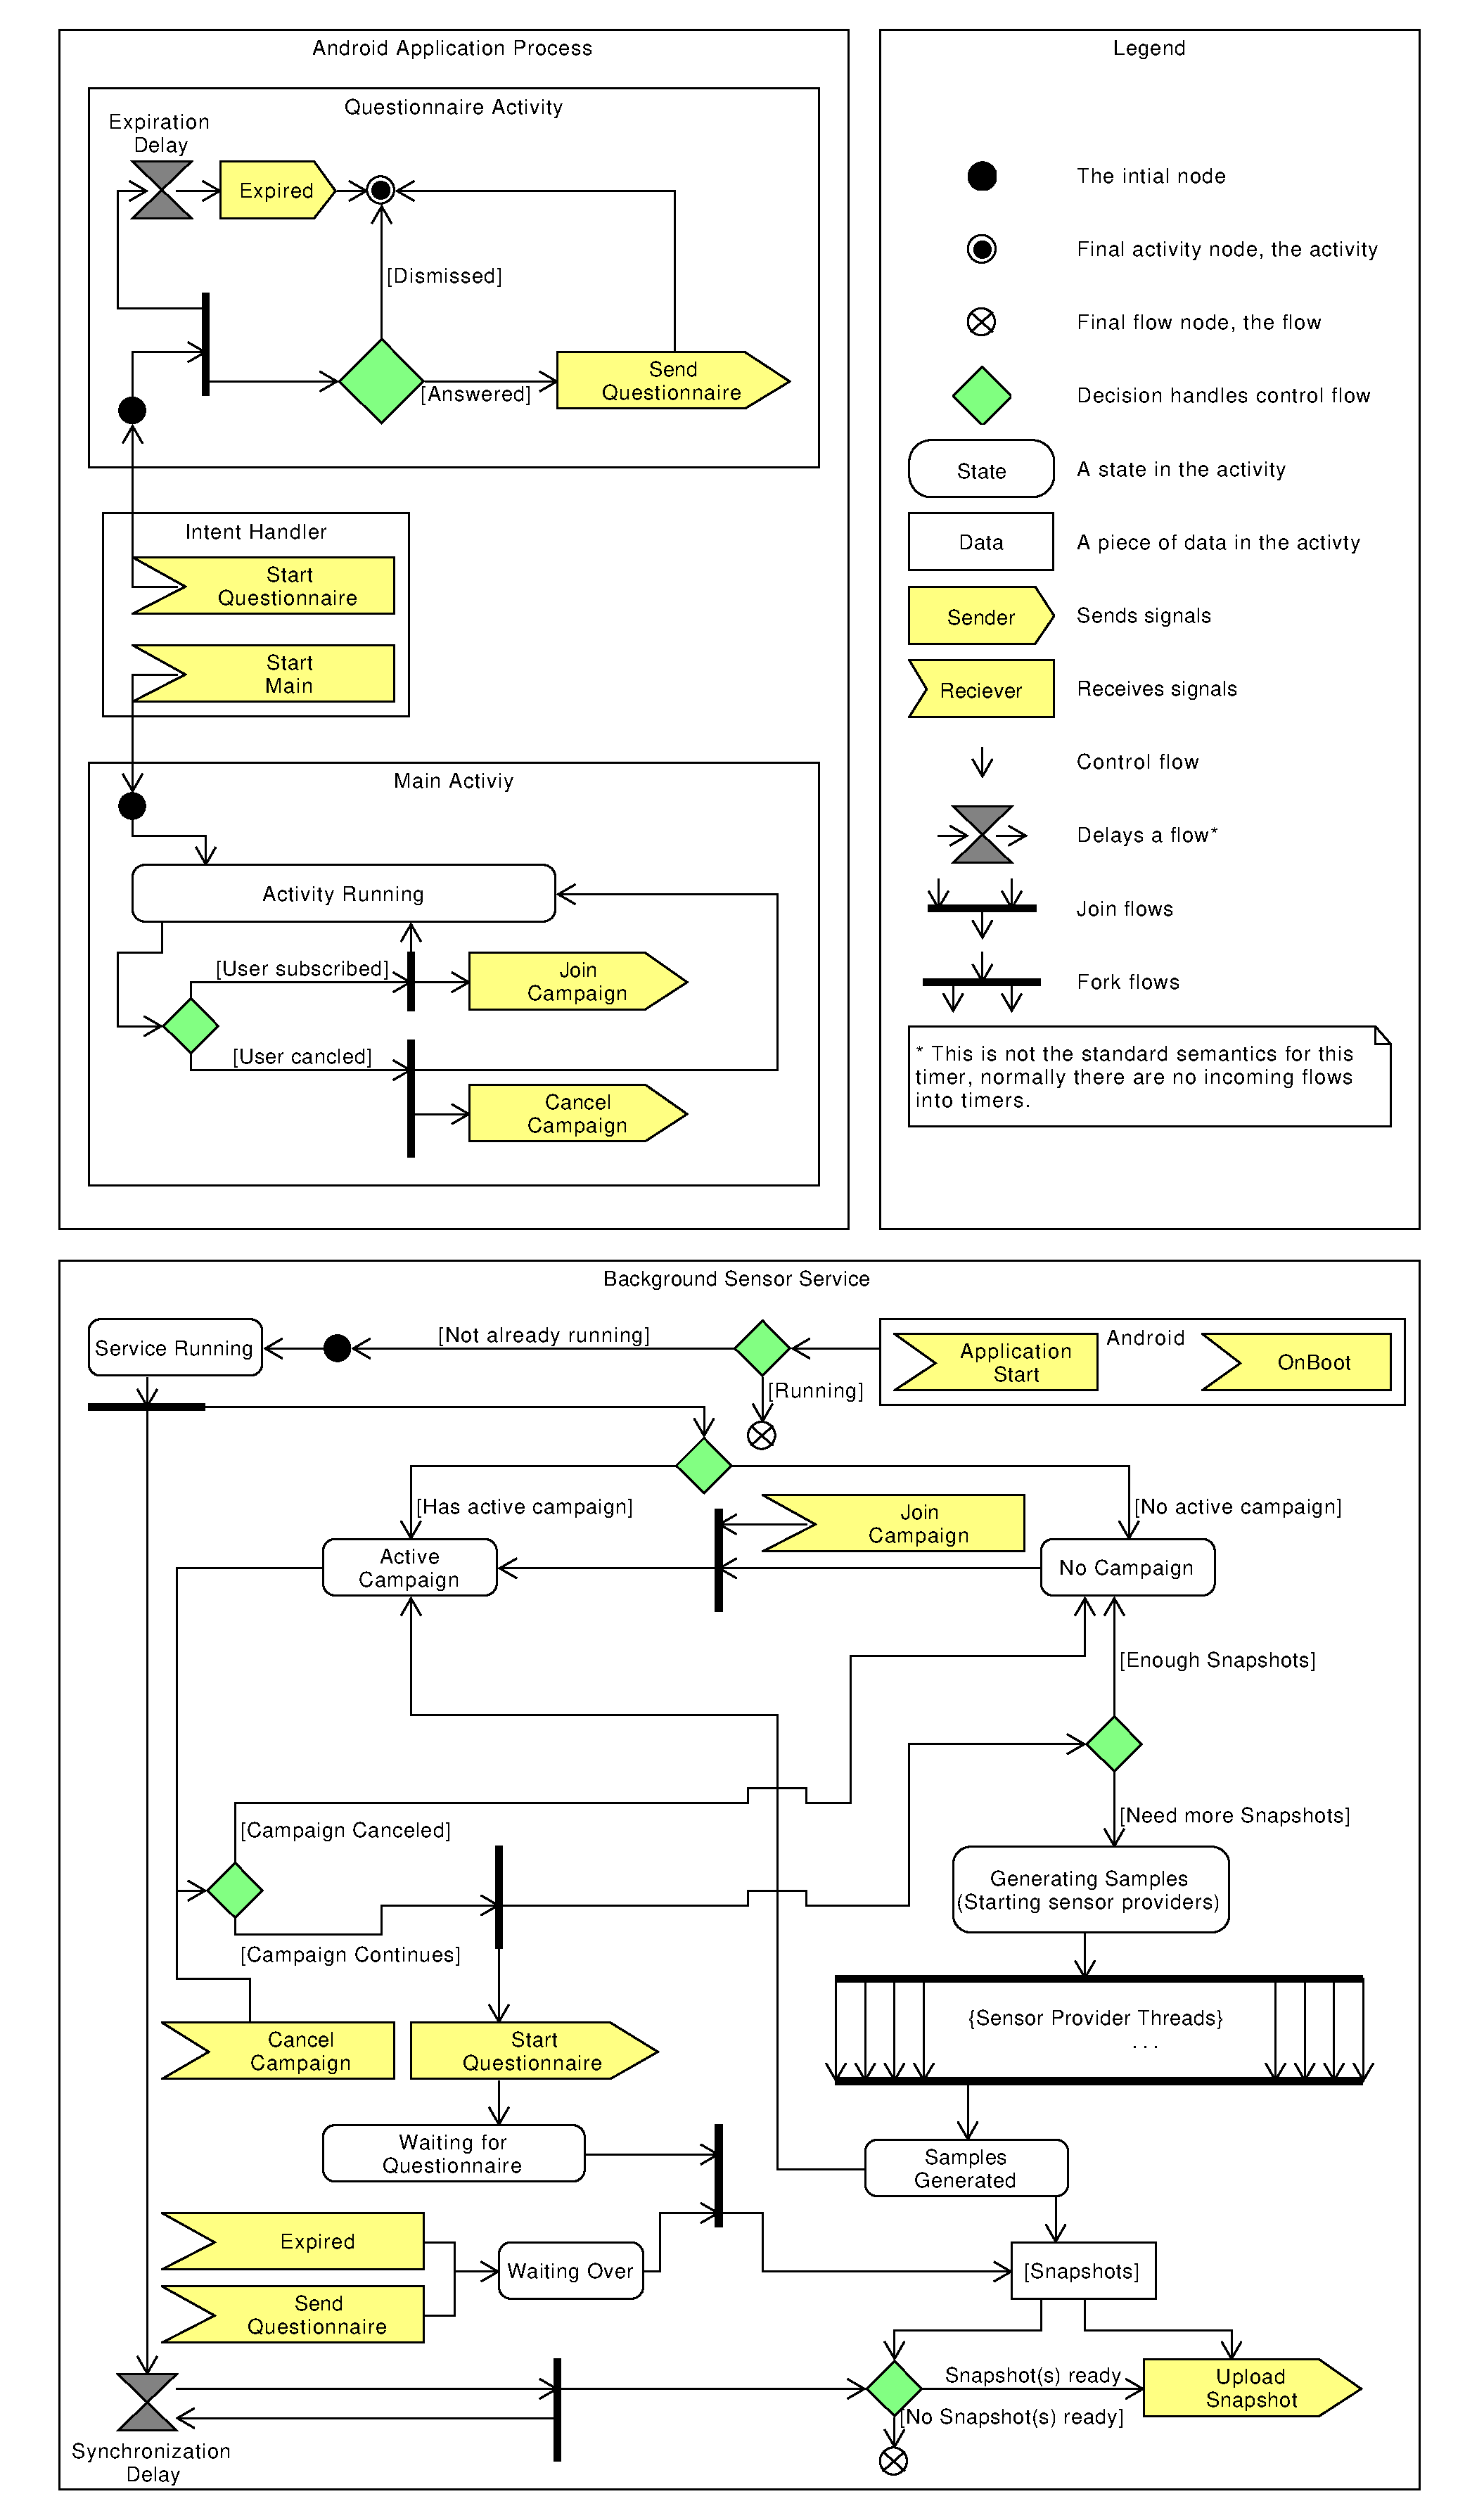
\includegraphics[width=0.9\textwidth]{graphic/backgroundsensorservice/lifecyclestuff}
    \caption{An overview of the mobile Application Components.}
    \label{fig:system_currency_and_lifecycle}
\end{figure}
\FloatBarrier